\lab{Applications}{Markov Chains I}{Markov Chains I}
\label{Ch:Markov}

\objective{This section teaches about two simple applications of Linear Algebra. First it teaches about Markov Chains, which in this context represent discrete random transitions. Second it teaches about Graph Theory, which can be used to represent many physical problems.}

\section*{Markov Chains}

%Lab \ref{Markov}

A Markov Chain describe a particular type of random variable. This type of random variable is characterized by the fact that all relevant information is related to its current state. We can easily model this type of random variable using matrices. We will start with a canonical example of a frog jumping from one lilypad to another.

Fredo the Frog hops around between the three lily pads $A$, $B$, and $C$.  If he's on lily pad $A$ and jumps, there is a 25\% chance that he will land back on lily pad $A$, a 25\% chance that he will land on lily pad $B$, and a 50\% chance that he will land on lily pad $C$.  In Figure `2.1, we have a transition diagram that reflects the various probabilities from which Fredo will go from one lily pad to another.

\begin{figure}[h!]
\label{markov1_fig1}
\begin{center}
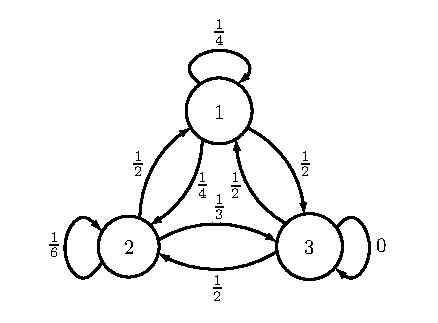
\includegraphics[scale = 1]{markov1}
\end{center}
\caption{Transition diagram for Fredo the Frog}
\end{figure}

We can convert our transition diagram into a transition matrix, where the $(i,j)$-entry of the matrix corresponds to the probability that Fredo jumps from the $j^{th}$ lily pad to the $i^{th}$ lily pad (where of course $A$ is the first lily pad, $B$ is the second, and so on).  In Fredo's case, the transition matrix is
\[
A = \begin{pmatrix}
1/4 & 1/2 & 1/2\\
1/4 & 1/6 & 1/2\\
1/2 & 1/3 & 0
\end{pmatrix}
\]
Note that all of the columns add up to one.  This is important.

If Fredo is on lily pad $A$, where will he be after two jumps?  By multiplying the matrix $A$ by itself, we have (approximately)

\[
A^2 = \begin{pmatrix}
0.4375 & 0.3750 & 0.3750\\
0.3542 & 0.3194 & 0.2083\\
0.2083 & 0.3056 & 0.4167
\end{pmatrix}
\]
From this, we infer that there is a 43.75\% chance he will still be on lily pad $A$ after two jumps.  Note that he might have jumped from $A$ to $A$ to $A$, denoted $A \rightarrow A \rightarrow A$, or he could have jumped to one of the other lily pads and then back again, that is, either $A \rightarrow B \rightarrow A$ or $A \rightarrow C \rightarrow A$.  In addition, there is a 35.42\% chance he will be on lily pad $B$ and a 20.83\% chance that he will be on lily pad $C$.  Using Python, we can type in our transition matrix and see where Fredo will be after 5, 10, 20 or 100 jumps.

\begin{lstlisting}[style=python]
#Remember, the 1.'s in the numerator force floating point division
: A = sp.array([[1./4,1./2,1./2],[1./4,1./6,1./2],[1./2,1./3,0]])
: np.linalg.matrix_power(A,5)
: np.linalg.matrix_power(A,10)
: np.linalg.matrix_power(A,20)
: np.linalg.matrix_power(A,100)
\end{lstlisting}

Note that in the limit that the number of jumps goes to infinity, we get
\[
A^\infty = \begin{pmatrix}
0.4 & 0.4 & 0.4\\
0.3 & 0.3 & 0.3\\
0.3 & 0.3 & 0.3
\end{pmatrix}
\]
This means that after several jumps, the probability that we will find Fredo on a given lily pad will have nothing to do with where he started initially.
 
\section*{Markov Chains}

We can generalize this notion beyond that of frogs and lily pads.  Let the state of our system be represented by a probability vector
\[
\x = \begin{bmatrix}
x_1\\
x_2\\
\vdots\\
x_n
\end{bmatrix}
\]
where each entry represents the probability of being in that state.  Note that each entry is nonnegative and the sum of all the entries adds up to one.  For example, in the case of Fredo, if we know initially that he is on lily pad $A$, then we have the state vector
\[
\x_0 = \begin{bmatrix}
1\\
0\\
0
\end{bmatrix}
\]
because we know for certainty (100\%) that Fredo is in the first state.  After one jump, we have
\[
\x_1 = A \x_0 = \begin{bmatrix}
0.25\\
0.25\\
0.50
\end{bmatrix}
\]
After two jumps, we have
\[
\x_2 = A \x_1 = A^2 \x_0 = \begin{bmatrix}
0.4375\\
0.3542\\
0.2083
\end{bmatrix}
\]
After a large number of jumps $(n>>1)$, we have
\[
\x_n = A \x_{n-1} = \dots = A^n \x_0 \approx \begin{bmatrix}
0.4\\
0.3\\
0.3
\end{bmatrix}
\]
Since all of the columns are the same for $A^\infty$, then for any initial probability vector $\x_0$, we get the same limiting output, or in other words, all initial vectors converge to the same point, call it $\x_\infty$.  Moreover, we have that
\[
\x_\infty = A \x_\infty
\]
This is called a stable fixed point.  How can we check that a stable fixed point exists?  Hint: Think eigenvalues and eigenvectors.

\section*{Example}

Consider the Markov chain given by
\[
A = \begin{pmatrix}
0.5 & 0.3 & 0.4\\
0.2 & 0.2 & 0.3\\
0.3 & 0.5 & 0.3
\end{pmatrix}.
\]
We show that it has a stable fixed point by checking that it has a single eigenvalue $\lambda=1$.  We do this via Python:
\begin{lstlisting}[style=python]
: A = sp.array([[.5,.3,.4],[.2,.2,.3],[.3,.5,.3]])
: V = la.eig(A)[1]
\end{lstlisting}
Note that the entries in the $\lambda=1$ eigenvector do not generally add up to one.  Indeed, any multiple of an eigenvector is an eigenvector.  So we need to multiply it by the appropriate constant so that all of the entries add up to one.
\begin{lstlisting}[style=python]
: x = V[:,0]
: x = x/sp.sum(x);x
array([ 0.41836735,  0.23469388,  0.34693878])
\end{lstlisting}
We can check this answer by taking $A$ to a high exponent, say $A^{100}$.

\begin{problem}
Suppose a basketball player's success at shooting free throws can be
described with the following Markov chain
\[
A = \begin{pmatrix}.75&.50\\.25&.50\end{pmatrix}
\]
where the first state corresponds to success and the second state to failure.
\begin{enumerate}
\item If the player makes his first free throw, what is the probability that he also makes his third one?
\item What is the player's average free throw percentage?
\end{enumerate}
\end{problem}

\begin{problem}
Consider the Markov process given by the transition diagram in Figure 2 below:
\begin{enumerate}
\item Find the transition matrix.
\item If the Markov process is in state $A$, initially, find the probability that it is in state $B$ after 2 periods.
\item Find the stable fixed point if it exists.
\end{enumerate}
\end{problem}

\begin{figure}[h!]
\begin{center}
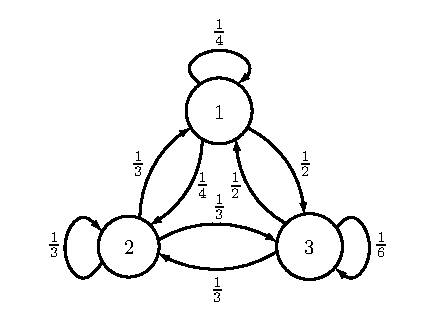
\includegraphics[scale = 1]{markov2}
\end{center}
\caption{Transition diagram}
\end{figure}

\newpage

\section*{Graph Theory}
\begin{center}
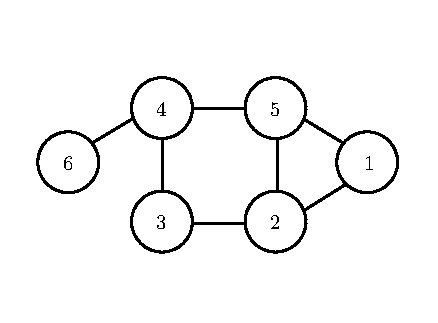
\includegraphics[scale = .8]{graphExample}
\end{center}

Graph theory is an important branch of mathematics and computer science. It describes how objects are connected to one another. In a rigorous sense, a graph is composed of two sets: a set of nodes and a set of edges that connect these nodes. 

A graph is directed if connections are uni-directional, and undirected if they are bi-directional. The above graphic shows an undirected graph. We can write a matrix that describes this type of graph. We let each row of our matrix represent our starting point and each column represent our destination. We put a 1 if there is a path and a 0 if there is not. For the above graph we generate the following matrix:

\[
A = \begin{pmatrix}
0 & 1 & 0 & 0 & 1 & 0\\
1 & 0 & 1 & 0 & 1 & 0\\
0 & 1 & 0 & 1 & 0 & 0\\
0 & 0 & 1 & 0 & 1 & 1\\
1 & 1 & 0 & 1 & 0 & 0\\
0 & 0 & 0 & 1 & 0 & 0
\end{pmatrix}
\]

This matrix is called an adjacency matrix. Note that this matrix is symmetric, since the graph is undirected.

What happens if we square an adjacency matrix? It turns out that raising an adjacency matrix to the n power yields the number of paths of length n between two vertices. For example by squaring the above matrix Python gives:
\begin{lstlisting}[style=python]
: np.linalg.matrix_power(A,2)
array([[2, 1, 1, 1, 1, 0],
       [1, 3, 0, 2, 1, 0],
       [1, 0, 2, 0, 2, 1],
       [1, 2, 0, 3, 0, 0],
       [1, 1, 2, 0, 3, 1],
       [0, 0, 1, 0, 1, 1]])
\end{lstlisting}

Now try to find the number of connections of length 6 from node 3 to itself. This is simple to do in Python:
\begin{lstlisting}[style=python]
: np.linalg.matrix_power(A,6)
array([[45, 54, 38, 45, 54, 16],
       [54, 86, 29, 77, 51, 11],
       [38, 29, 55, 15, 70, 27],
       [45, 77, 15, 75, 31,  4],
       [54, 51, 70, 31, 93, 34],
       [16, 11, 27,  4, 34, 14]])
\end{lstlisting}
It turns out that there are 55 unique paths of length 6 from node 3 to itself. Imagine trying to count all of those paths by hand! It would be very easy to count incorrectly. However, this method makes it very simple to count paths without any mistakes.

The astute reader may ask now why this matters. It turns out that the study of graphs and connectivity have many important applications. For example, connections between web pages can be described as graphs. So can flights between airports or friends on social networking sites. The same ideas are applied frequently in computer chip design and in the preservation of endangered species. We will explore one surprising application to chemistry.

Remeber the \li{bucky} array we explored in chapter one? The graph that this matrix represents is a graph for a geodesic dome, which has structure almost identical to certain types of carbon atoms. Understanding the graphs of certain types of molecules allows scientists to better understand the structure of the molecule, making identification and manipulation easier.

We will manipulate the matrix the \li{bucky} to simulate the types of analysis a scientist could do on a complex carbon atom. For our purposes, each column and row of the \li{bucky} matrix represents an atom in our molecule, and connections are chemical bonds from one atom to another.

\begin{problem}
Find the number of connections between atoms in our molecule(the command \li{sp.count\_nonzero} may be useful). Then find the number of atoms that are connected by paths of length two. Three? At what path length are all of the atoms connected?
A nifty way to visualize this is the \li{plt.spy} command. Read the documentation for \li{plt.spy} and then use \li{plt.spy} to visualize how the graph is connected at path length one, two, four and ten. Remember, to load \li{``bucky.csv''} into an array use the command \lstinline{bucky = sp.loadtxt ( "bucky.csv" , delimiter = "," )}.
\end{problem}
